\chapter{Dynamic Modeling of a Quadrotor}
\label{Dynamic_Modeling_of_a_Quadrotor}
\setcounter{MaxMatrixCols}{20}

This chapter describes the modeling efforts made to develop a suitable representation of the system for the MPC library developed, based on the physical phenomena responsible for the quadrotor's operation. To start, the theoretical derivation of the quadrotor model is exposed. To verify the correct behavior of the derived model, a section is dedicated to the verification tests and their respective results. A global summary is included at the end of the chapter to compile and discuss the achievements made.

\begin{figure}[h!]
\centering
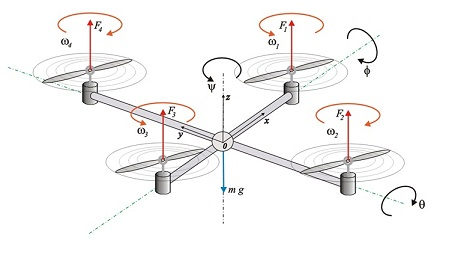
\includegraphics{Images/Chapter3/quad_dynamics.jpg}
\caption{Functioning scheme for the quadrotor dynamics. (Taken from \url{http://www.pupin.rs/RnDProfile/research-topic28.html})}
\label{fig:quadrotor_dynamics}
\end{figure}

A quadrotor has all six degrees of freedom in space and it has four actuators, which makes it an underactuated system. This means that two of the degrees of freedom must be controlled by means of regulating the other four in a proper manner. The four rotors are coupled, so the motion in the different directions is controlled by the difference in angular speed of the pairs of rotors. In Figure \ref{fig:quadrotor_dynamics}, the rotors are numbered so the pairs are defined in the directions of the axes. In order to move in the X axis, an imbalance must be made between the forces exerted by rotors 1 and 3, thus meaning a difference of angular speed in these rotors. It works the same way with the Y axis, as rotors 2 and 4 must be imbalanced as well to generate a motion in this direction. Notice that the changes in roll ($\phi$), pitch ($\theta$) angles are required to generate the motion in the X or Y directions. In order to move in the Z axis, all four rotors shall act in the same direction, therefore all four rotors must increase or decrease their angular speed. To perform a yaw ($\psi$) movement, the imbalance comes from both pairs, this is, rotors 2 and 4 rotate with a different angular speed than 1 and 3, since they rotate in opposite directions to cancel the rotating forces from the pairs and enable the quadrotor to \emph{hover} or standing still in the air.	


\section{Theoretical Derivation of the Quadrotor Model}

All known physical phenomena is used in order to obtain the theoretical model, however, the model can be as extensive as desired: in \cite{MahoneyKumarCorke2012}, the rotor aerodynamics and the concepts related to blade theory (drag and lift coefficients) are taken into consideration, however, other authors have chosen to reduce the system to use the model for control design, since these models depend on aerodynamic forces and torques, which are subjected to disturbances caused by winds and turbulence. In \cite{Hoffmann2007}, a more detailed study of the aerodynamic effects present in the quadrotor is made, but this kind of modeling is out of the scope of this report. In \cite{Bouabdallah2004} Bouabdallah et Al. state that the main physical effects present in the quadrotor system are mentioned and theoretically formulated, from which we can mention aerodynamic effects, inertial counter torques, gyroscopic effects, gravity effects and friction. However, the main effects to include for a simple model should be the gyroscopic effects of the rigid body rotation in space and the effects of the four propeller's rotation. \\

Let {$A$} and {$B$} denote two coordinate frames, where {$A$} is fixed to the ground and {$B$} is fixed to the quadrotor body in its gravity center. The relation between these two coordinate frames is defined by an homogeneous transformation given by the Euler angles, that in our case are the same angles used to determine the orientation of an airbourne vehicle: roll ($\phi$), pitch ($\theta$) and yaw ($\psi$). The transformation between {$A$} and {$B$} is defined by a rotation matrix given by the aforementioned angles and a translation vector measured from {$A$} to {$B$} as follows: 

\begin{equation} \label{eq:transformation}
\begin{pmatrix} x_A \\
				y_A \\
				z_A \end{pmatrix} = \mathbf{R_{A}^{B}}\begin{pmatrix} x_B \\
															  y_B \\
															  z_B \end{pmatrix} + \mathbf{t_{A}^{B}} 
\end{equation}

Where $\mathbf{R_{A}^{B}}$ and $\mathbf{t_{A}^{B}}$ are the rotation matrix from {$A$} to {$B$} and the translation vector from  {$A$} to {$B$}, respectively. The rotation matrix is defined as follows:

\begin{equation} \label{eq:rotationmatrix}
\mathbf{R_{A}^{B}} = \begin{bmatrix} \cos(\psi)\cos(\theta) & $\cos(\theta)\sin(\psi)$ & $ -\sin(\theta)$ \\
$\cos(\psi)\sin(\phi)\sin(\theta) - \cos(\phi)\sin(\psi)$ & $\cos(\phi)\cos(\psi) + \sin(\phi)\sin(\psi)\sin(\theta)$ & $\cos(\theta)\sin(\phi)$ \\
$\sin(\phi)\sin(\psi) + \cos(\phi)\cos(\psi)\sin(\theta)$ & $\cos(\phi)\sin(\psi)\sin(\theta) - \cos(\psi)\sin(\phi)$ & $\cos(\phi)\cos(\theta)$ \end{bmatrix}
\end{equation}

And the translation vector is simply defined as the position vector from the inertial frame ${A}$ to the body frame ${B}$. This rotation and translation together define a homogeneous transformation \textbf{T} as in equation {\ref{eq:homogeneoustransform}}.

\begin{equation} \label{eq:homogeneoustransform}
\mathbf{T_{A}^{B}} = \begin{bmatrix} \mathbf{R_{A}^{B}} & \mathbf{t_{A}^{B}} \\ 0 & 1 \end{bmatrix}
\end{equation}

If $\mathbf{v} \in A$ is the velocity of the body frame {$B$} expressed in {$A$}, $\boldsymbol{\Omega} \in B$ is the rotational velocity of the angular frame {$B$} with respect to {$A$}, expressed in {$B$}, $m$ is the quadrotor's mass and $\mathbf{I} \in \mathbb{R}^{3 \times 3}$ is the inertia matrix expressed in the body fixed frame {$B$}; a Newton's second Law of Motion force and torque balance, together with the kinematic relations between the frames lead to the following formulation:

\begin{equation} 
\begin{subequations} \label{eq:newtonformulation}
\begin{align}
	\dot{\mathbf{t}} &= \mathbf{v} \label{first}\\
	m\dot{\mathbf{v}} &= mg\hat{\mathbf{k_A}} + R\mathbf{F} \label{second}\\
	\dot{R} &= R\Omega\times\mathbf{v} \label{third}\\
	\mathbf{I}\dot{\boldsymbol{\Omega}} &= -\boldsymbol{\Omega}\times\mathbf{I}\boldsymbol{\Omega} + \boldsymbol{\tau} \label{fourth}
\end{align}
\end{subequations}
\end{equation}

When the system is expanded as scalar equations, the resultant is a 12 equation system as follows:

\begin{equation} 
\begin{subequations} \label{eq:newtonformulationexpanded}
\begin{align}
	\dot{x} &= u \label{first}\\
	\dot{y} &= v \label{second}\\
	\dot{z} &= w \label{third}\\
	\dot{u} &= \frac{1}{m}(\cos{\psi}\sin{\theta}\cos{\phi} + \sin{\psi}\sin{\phi})\mathbf{F} \label{fourth}\\
	\dot{v} &= \frac{1}{m}(\sin{\psi}\sin{\theta}\cos{\phi} - \cos{\psi}\sin{\phi})\mathbf{F} \label{fifth}\\
	\dot{w} &= \frac{1}{m}(\cos{\theta}\cos{\phi})\mathbf{F} - g\label{sixth}\\
	\dot{\phi} &= \dot{p} + q\sin{\phi}\tan{\theta} +r\cos{\phi}\tan{\theta} \label{seventh}\\
	\dot{\theta} &=  q\cos{\phi} - r\sin{\phi}\label{eighth}\\
	\dot{\psi} &= q\sin{\phi}\sec{\theta} + r\cos{\phi}\sec{\theta}\label{nineth}\\
	\dot{p} &= \frac{(I_{yy} - I_{zz})}{I_{xx}}qr - \frac{J_R\Omega}{I_{xx}}q + \frac{l}{I_{xx}}\boldsymbol{\tau_{\phi}}\label{tenth}\\
	\dot{q} &= \frac{(I_{zz} - I_{xx})}{I_{yy}}pr + \frac{J_R\Omega}{I_{yy}}p + \frac{l}{I_{yy}}\boldsymbol{\tau_{\theta}}\label{eleventh}\\
	\dot{q} &= \frac{(I_{xx} - I_{yy})}{I_{zz}}pq + \frac{1}{I_{zz}}\boldsymbol{\tau}_{\psi} \label{twelveth}\\
\end{align}
\end{subequations}
\end{equation}

Where $\mathbf{F}$ and $\boldsymbol{\tau}$ are vectors expressed in {$B$} that represent all the external forces and torques made by the aerodynamics of the rotors. These aerodynamic effects have been studied in \cite{Hoffmann2007} in depth, although this approach is unpractical in a robotics context. Nevertheless, some aerodynamics will be covered in this section to get a model that interacts at actuator level, this is, uses properties of the actuators as states. \\

For this equations system, the natural selection for the states is to choose linear and angular positions and velocities, since the derivatives of these are given in the left hand side of the set of equations 3.7. It is important to notice that these angular velocities are not equal to the derivative of the Euler angles in the mobile frame {$B$}. The derivative of the Euler angles is a discontinuous function. On the other side, the angular velocities in the mobile frame {$p, q, r$} are directly measurable through the Inertial Measurement Unit of the quadrotor, as it's actually done. From these measurements, the Euler angles are calculated \cite{Raffo2007}. Therefore we obtain a system with 12 states, as follows:

\begin{equation} \label{eq:statevector}
\mathbf{X} = \begin{bmatrix} x & y & z & u & v & w & \phi & \theta & \psi & p & q & r \end{bmatrix}
\end{equation} 

As of right now, the model takes as input the upward force coming from the combination of the thrust of the four rotors, and the three torques in space that command the orientation and angular velocities of the quadrotor frame. These quantities are difficult to measure and knowing the relationship between the rotational speeds of the actuators and these forces and torques, it is easier to think in a model where the inputs are the angular velocities of the rotors. The thrust provided by a single rotor is given by \cite{MahoneyKumarCorke2012} according to momentum theory:

\begin{equation} \label{eq:rotorthrust}
T_i = C_T\rho A_{r_{i}}r_{i}^2 \bar{\omega}^2
\end{equation}	

Where $C_T$ is the thrust coefficient for that rotor blade geometry and profile, $\rho$ is the density of air, $A_{r_{i}}$ is the rotor disk area and $\omega$ is the angular velocity. In order to perform a simpler and more practical identification, a simplified lumped-parameters model can be determined by static thrust experiments, as shown in equation \ref{eq:thrustsimple} :

\begin{equation} \label{eq:thrustsimple}
T_i = c_T \bar{\omega}^2
\end{equation}

For the case of the quadrotor, the forces and torques in space that influence the system can be decomposed in terms of the rotational speeds as follows:

\begin{equation} \label{eq:thrust_aerodynamics}
\begin{subequations}
\begin{align}
	\mathbf{F} &= c_T\bar{\omega}_1^2 + c_T\bar{\omega}_2^2 + c_T\bar{\omega}_3^2 + c_T\bar{\omega}_4^2 \label{first}\\
	\mathbf{\tau_{\phi}} &= dc_T(\bar{\omega}_2^2 - \bar{\omega}_4^2) \label{second}\\
	\mathbf{\tau_{\theta}} &= dc_T(\bar{\omega}_3^2 - \bar{\omega}_1^2) \label{third}\\
	\mathbf{\tau_{\psi}} &= c_Q((\bar{\omega}_2^2 + \bar{\omega}_4^2) - (\bar{\omega}_1^2 + \bar{\omega}_3^2)) \label{fourth}
\end{align}
\end{subequations}
\end{equation}
	
Obtaining this simplified model experimentally has the advantage that the $c_T$ coefficient includes the drag effect on the airframe that is induced due to the airflow caused by the rotor. For this model of the quadrotor, more detailed identification experiments were performed by \cite{YueSun2012}, from which the resulting parameters are taken. \\

Due to the transformation matrix, the previously presented model of the system is non-linear, and since the solver requires a linear representation, a linearization process is required. This linearization process is done using the truncated approximation to Taylor series around a certain linearization point. The performance of this model will decrease when going away from this operation point, and therefore for the purposes of MPC, the accuracy of the predictions in these cases will not be as good. There are several ways to improve this, like selecting operation points distributed around the known regions of operation of the model, so it will change the information being used depending on its current state. Another alternative is to use a variable operation point that is changed in every single iteration so the model is always in the operation point. This strategy has the downside that it implies that the system matrices will be recalculated on every iteration, consuming computational resources. The operation point used for the validation tests is presented below. This point corresponds to the quadrotor in a hover state at a determined height $z$ correspondent with the desired height of the test. 

\begin{equation*} \label{eq:operationpoint}
\mathbf{X}^* = \begin{bmatrix} 0 & 0 & z & 0 & 0 & 0 & 0 & 0 & 0 & 0 & 0 & 0 \end{bmatrix}
\end{equation*} 

Since the objective of this thesis is not focused on modeling, a simple model with a static operation point will be used for demonstration together with the MPC software. This will have its effect on the performance of the MPC, but this effect can be reduced in some level by increasing the prediction horizon, at the cost of generating a bigger quadratic problem to solve. However, the computer running this simulation has enough processing power to handle it, but this should be highly regarded when performing this task on an onboard computer.

\section{Verification of the Model}

It is important to clarify that the following work consists only in verification, without validation. When the model is verified, its behavior is assesed to be correct, according to the described by the equations that rule the quadrotor's dynamics. However, it is not validated, in the sense that it is not proven that the model describes the behavior of the real platform. This work was not performed because the available AR Drone quadrotor takes as inputs velocity commands to an unknown control scheme programmed in the quadrotor's processing unit. Unveiling the inner control scheme in the quadrotor and bypassing it is a task that for time reasons is not performed, and therefore, the model will be simulated with the parameters identified in \cite{YueSun2012}. 

\begin{equation} \label{eq:statevector}
\mathbf{X} = \begin{bmatrix} x & y & z & u & v & w & \phi & \theta & \psi & p & q & r \end{bmatrix}
\end{equation} 

There will be two simulations performed: one with the linearized model and one with the whole non-linear model of the platform. This is useful for the application in the MPC, where it is required to have one linear model for the platform to perform the predictions and set the quadratic problem, and the simulator for the platform, that will be represented by the full non-linear model in order to have more realistic simulations. \\

The following experiments show the outputs of the systems when a predefined set of inputs is given. These inputs are designed to obtain a specific movement pattern characteristic of the quadrotor in order to be able to analyze the outputs and assess the correctness of the outputs.These movements are the following: upwards motion along the $Z$ axis, lateral and frontal movement around the $X,Y$ axes respectively, and yaw rotation. 

\subsection{Upward motion along the Z axis}

In order to generate the thrust to elevate the quadrotor, the rotors must be all operating at the same speed, above the equilibrium rotational speed (which is around 360 rad/s). 
\begin{equation} \label{eq:statevector}
\mathbf{X} = \begin{bmatrix} x & y & z & u & v & w & \phi & \theta & \psi & p & q & r \end{bmatrix}
\end{equation} 
\begin{figure}[h!]
\centering
\includegraphics[scale=0.7]{Images/Chapter3/Constant_thrust_upwards/Inputs_UP.png}
\caption{Inputs to generate an upward motion of the quadrotor.}
\label{fig:upwards_inputs}
\end{figure}

In Figure \ref{fig:upwards_inputs}, the used input signal to the model can be observed. The desired motion is an initial elevation of the quadrotor followed by a descent to some point. Therefore the signal follows this pattern. The resulting plots show the response of the simulated systems. 

\begin{figure}[h!]
\centering
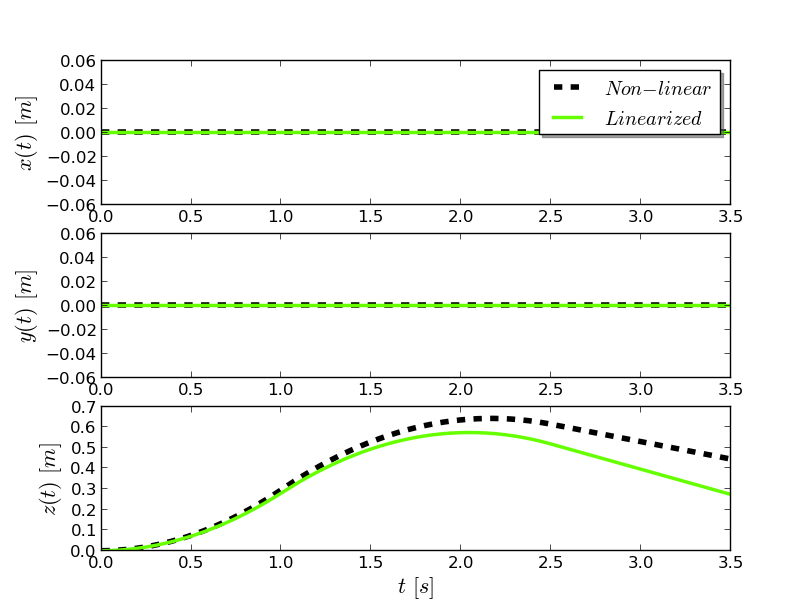
\includegraphics[scale=0.7]{Images/Chapter3/Constant_thrust_upwards/Positions.png}
\caption{Resulting positions of the simulated systems for the given inputs.}
\label{fig:upwards_positions}

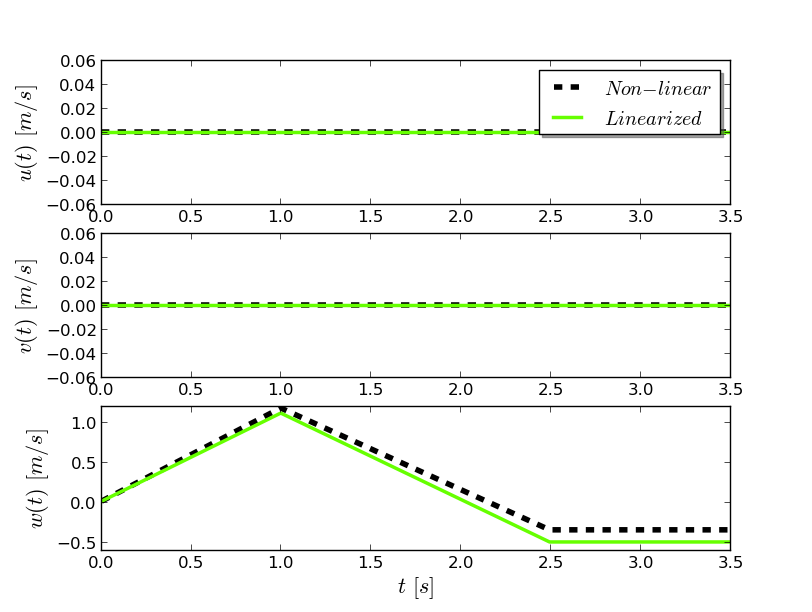
\includegraphics[scale=0.7]{Images/Chapter3/Constant_thrust_upwards/Linear_velocities.png}
\caption{Resulting velocities of the simulated systems for the given inputs.}
\label{fig:upwards_velocities}
\end{figure}

The plots for the Euler angles and the angular velocities are not shown because in this movement the angular variables are not changing. The behavior obtained is the expected in both cases, with the differences between them being caused by the linearization process. We can see that as the linear model goes further away from the linearization point the performance decreases in comparison to the non-linear model that is used as a performance reference. It is to notice that this is a simulation that doesn't take into account the ground. In Figure \ref{fig:upwards_velocities}, the velocity goes to negative values because the time that the signal goes under the equilibrium rotational speed is bigger than the time that the thrust is active, and when the equilibrium is achieved, the model keeps the negative velocity. The behavior is correct, but the absence of ground makes room for this kind of details that might confuse when verifying. 

\subsection{Lateral movement along the X axis}

To move the quadrotor in the $XY$ plane, a difference in the rotor speed between the pair (1,3) must be produced as seen from equation 3.12, so the pitch torque increases and tilts the frame sideways. The design goal for the input signal was to imitate the inner controller loop in the quadrotor, since the modeling only considers the physical equipment without any control, and this system configuration is open-loop unstable. However, because of this, the signal must restore the system to its equilibrium state. The signal was obtained in an empirical way, based on the linearized and non-linear expressions that describe the system. \\

The resultant signal is a collection of pulses in opposite directions to counter each other and create the restoration effect. To have a better understanding of the effect of the signal on the model, the mapping between rotor speeds and thrust and torques acting on the quadrotor frame has been made and plotted and added below.

\begin{figure}[h!]
\centering
\includegraphics[scale=0.7]{Images/Chapter3/Lateral_X/Inputs_X.png}
\caption{Rotor speed inputs to generate a lateral movement along the X axis on the quadrotor.}
\label{fig:lateralX_inputs}
\end{figure}

\begin{figure}[H]
\centering
\includegraphics[scale=0.7]{Images/Chapter3/Lateral_X/Torque_inputs_X.png}
\caption{Rotor speed inputs from Figure \ref{fig:lateralX_inputs} mapped into forces and torques acting in the quadrotor frame.}
\label{fig:lateralX_torqueinputs}
\end{figure}


\begin{figure}[h!]
\centering
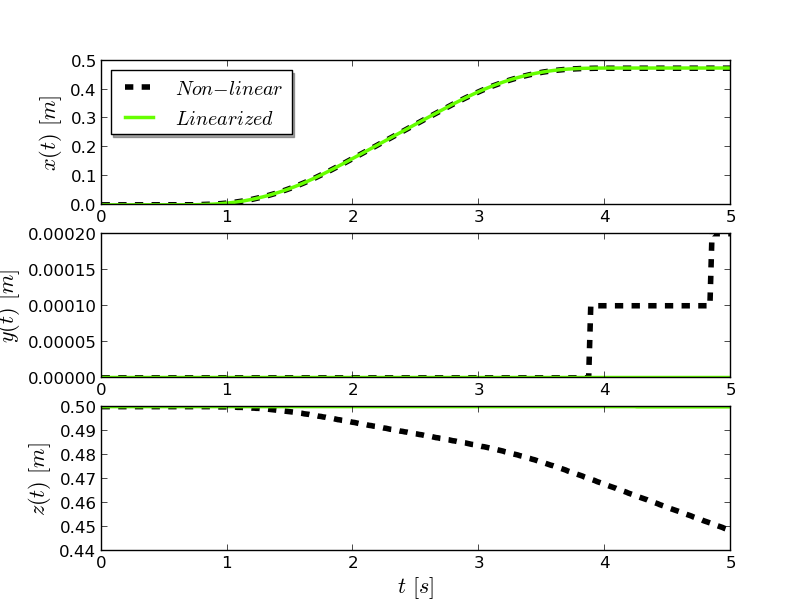
\includegraphics[scale=0.7]{Images/Chapter3/Lateral_X/Positions.png}
\caption{Resulting positions of the simulated systems for the inputs shown in Figure \ref{fig:lateralX_inputs}.}
\label{fig:LateralX_positions}

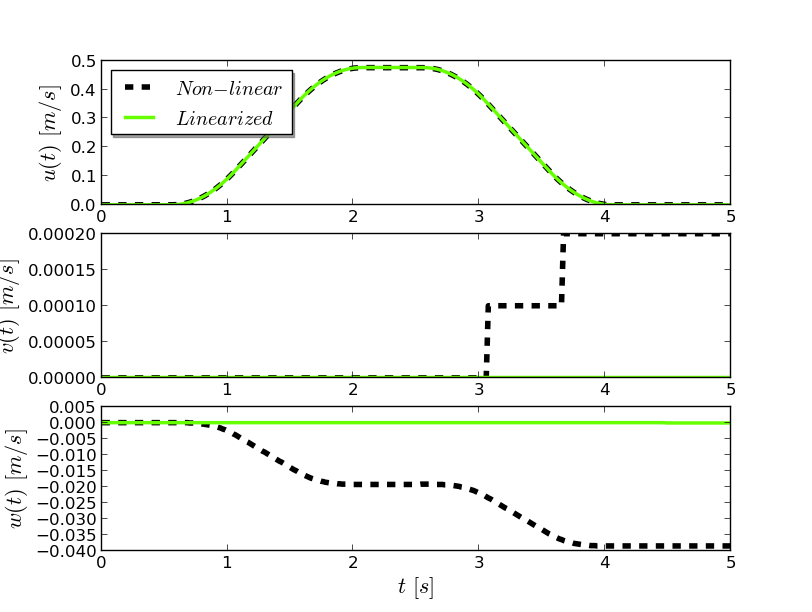
\includegraphics[scale=0.7]{Images/Chapter3/Lateral_X/Linear_velocities.png}
\caption{Resulting velocities of the simulated systems for the inputs shown in Figure \ref{fig:lateralX_inputs}.}
\label{fig:LateralX_velocities}
\end{figure}

\begin{figure}[h!]
\centering
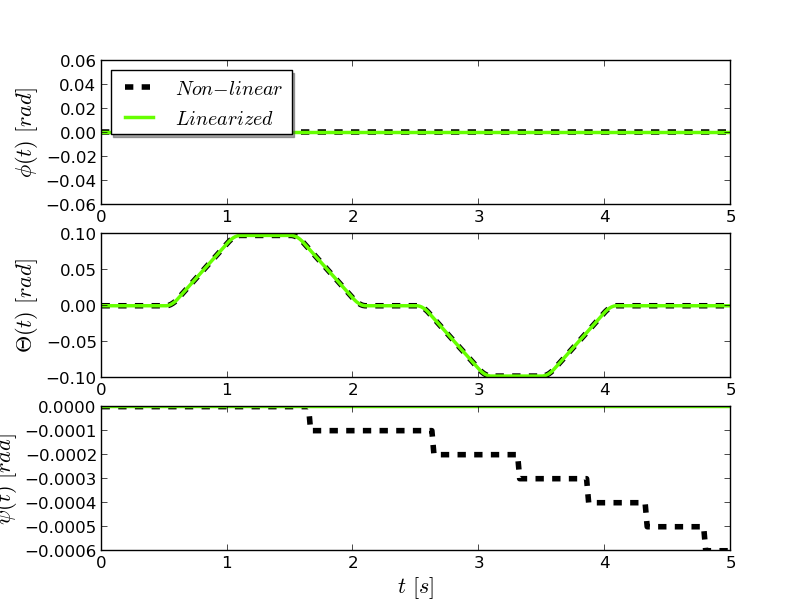
\includegraphics[scale=0.7]{Images/Chapter3/Lateral_X/Euler_Angles.png}
\caption{Resulting Euler angles of the simulated systems for the inputs shown in Figure \ref{fig:lateralX_inputs}.}
\label{fig:LateralX_Euler}

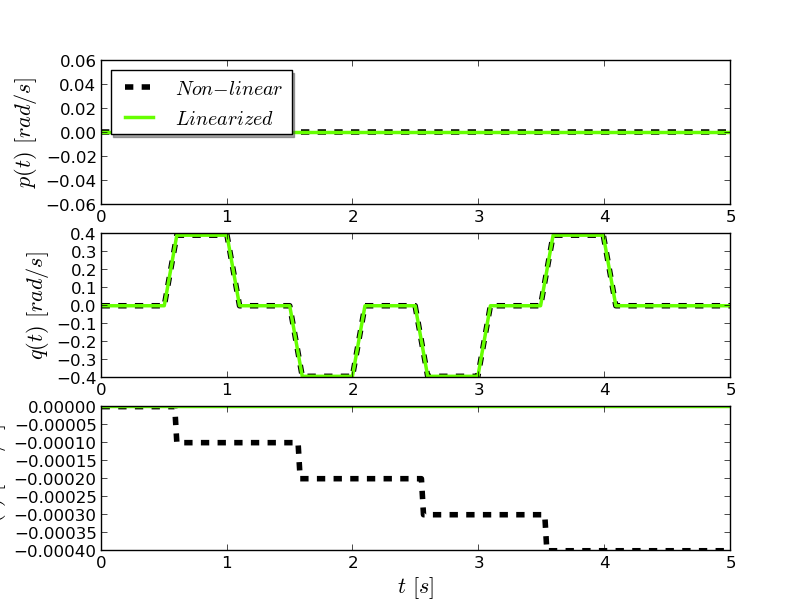
\includegraphics[scale=0.7]{Images/Chapter3/Lateral_X/Angular_velocities.png}
\caption{Resulting angular velocities of the simulated systems for the inputs shown in Figure \ref{fig:lateralX_inputs}.}
\label{fig:LateralX_angvelocities}
\end{figure}

In this simulation the quadrotor is starting from a determined height of $0.5$ meters. The resulting behavior of the model is quite satisfactory for this particular control signal. The difference between the linearized and the non-linear model is barely noticeable because the main non-linearities are introduced by the roll and pitch angles, which are kept in a very small range. Therefore, one could consider that $\cos{(\alpha)} \approx 1$ and $\sin{(\alpha)} \approx 0$. The torque inputs seen in Figure \ref{fig:lateralX_torqueinputs} are the ones calculated without the linearization process. Therefore, when a difference between a pair of rotors is stablished, there is also a slight change in the thrust, because the difference is squared. However, this difference is too small to influence the platform. This is not noticeable in the linearized output torque inputs. Another observation to highlight is that any movement of the quadrotor in any direction of the $XY$ plane will decrease a little bit the $Z$ coordinate because the thrust is redistributed for lateral movement. 

\subsection{Lateral movement along the Y axis}

The same input signals designed for the previous test are used in this case, only that they are applied in the (2,4) pair of rotors to switch axes.

\begin{figure}[H]
\centering
\includegraphics[scale=0.7]{Images/Chapter3/Lateral_Y/Inputs_Y.png}
\caption{Rotor speed inputs to generate a lateral movement along the Y axis on the quadrotor.}
\label{fig:lateralY_inputs}
\end{figure}

\begin{figure}[H]
\centering
\includegraphics[scale=0.7]{Images/Chapter3/Lateral_Y/Torque_inputs_Y.png}
\caption{Rotor speed inputs from Figure \ref{fig:lateralY_inputs} mapped into forces and torques acting in the quadrotor frame.}
\label{fig:lateralY_torqueinputs}
\end{figure}


\begin{figure}[h!]
\centering
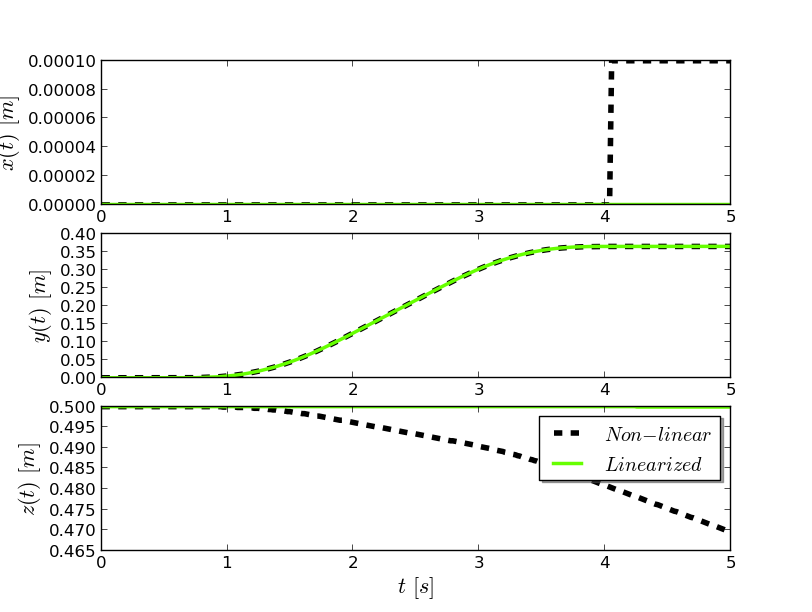
\includegraphics[scale=0.7]{Images/Chapter3/Lateral_Y/Positions.png}
\caption{Resulting positions of the simulated systems for the inputs shown in Figure \ref{fig:lateralY_inputs}.}
\label{fig:LateralY_positions}

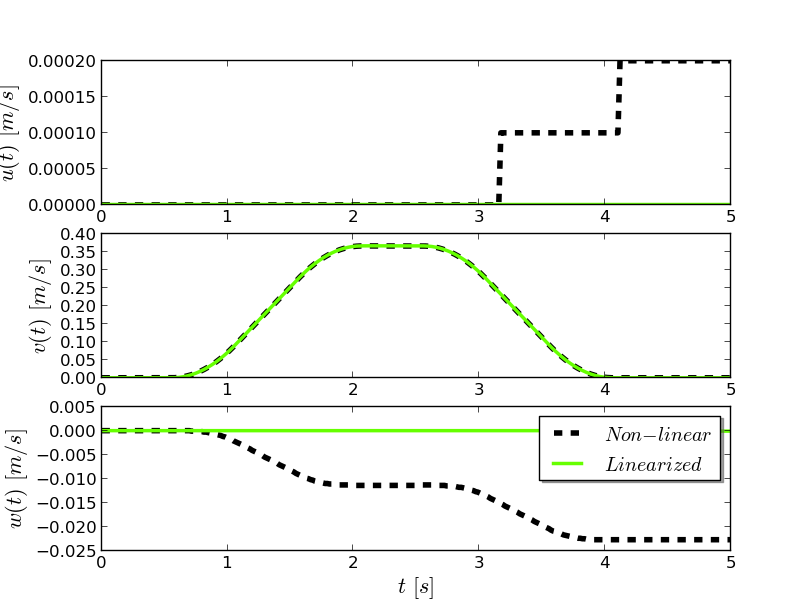
\includegraphics[scale=0.7]{Images/Chapter3/Lateral_Y/Linear_velocities.png}
\caption{Resulting velocities of the simulated systems for the inputs shown in Figure \ref{fig:lateralY_inputs}.}
\label{fig:LateralY_velocities}
\end{figure}

\begin{figure}[h!]
\centering
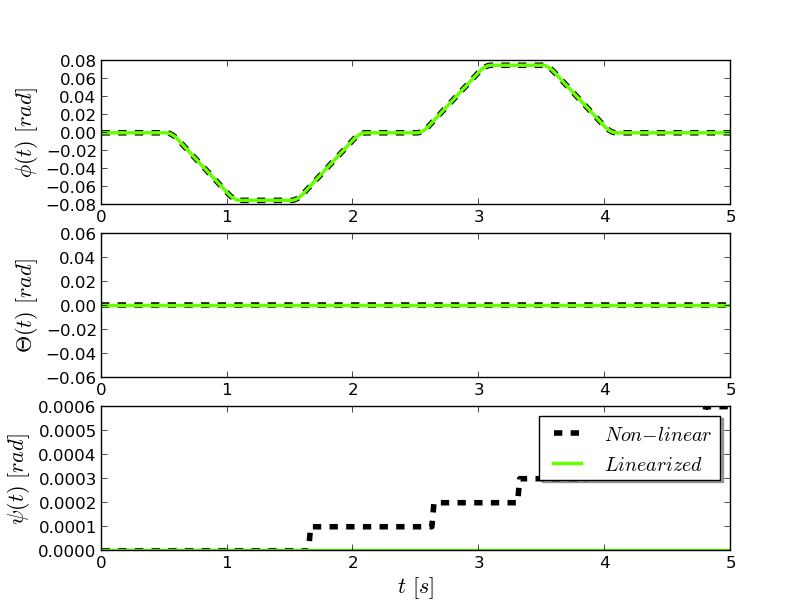
\includegraphics[scale=0.7]{Images/Chapter3/Lateral_Y/Euler_Angles.png}
\caption{Resulting Euler angles of the simulated systems for the inputs shown in Figure \ref{fig:lateralY_inputs}.}
\label{fig:LateralY_Euler}

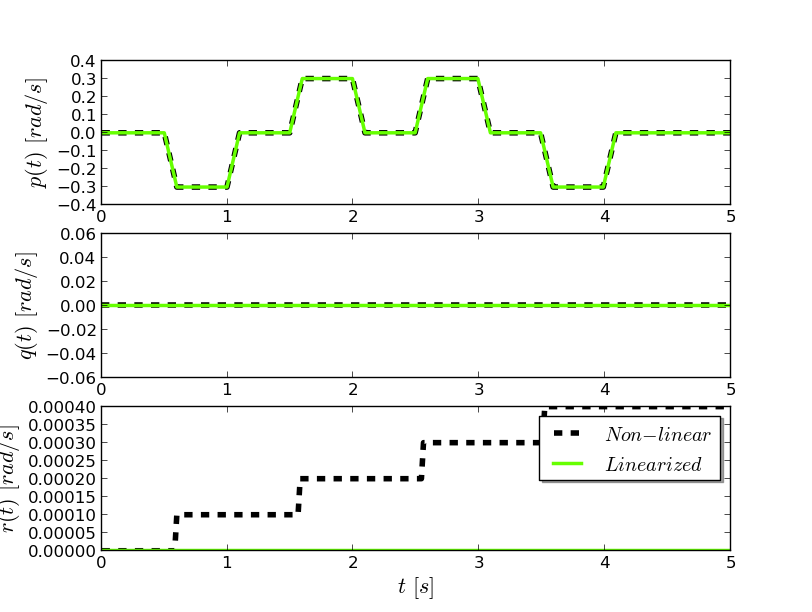
\includegraphics[scale=0.7]{Images/Chapter3/Lateral_Y/Angular_velocities.png}
\caption{Resulting angular velocities of the simulated systems for the inputs shown in Figure \ref{fig:lateralY_inputs}.}
\label{fig:LateralY_angvelocities}
\end{figure}

The resulting outputs have the same properties as the ones observed for the movement along the $X$ axis: a descent in the $Z$ coordinate caused by the coupling of the thrust force and very similar behavior between the linearized and non-linear model. In Figure \ref{fig:LateralY_positions} one can notice that the total displacement in the $Y$ axis is a little bit less in this direction, because this direction is sideways and the protective hull of the quadrotor has a bigger cross section area along this axis. 
\newpage

\section{Summary}

In this chapter a linear model of the quadrotor has been derived to integrate with the MPC software solution. This model is derived from the theoretical description of the physical phenomena responsible for the movement of the quadrotor. The quadrotor being modelled, Parrot's AR-Drone, has an inner control loop that includes the user. This is not taken in consideration in the derivation of this model. The model takes the angular speeds of the rotors as inputs and provides the quadrotor's position and yaw angle as outputs. The selection of the outputs correspond to the states being controlled, as it will be addressed later in the report. The model is linear due to a linearization process based on Taylor's series approximation, centered around a single operation point. The resulting model behaves good for small variations from this operation point. The input signals designed for the verification tests take into account that the model is open-loop unstable, so a restoring effect was required in order to obtain results that are easier and more intuitive to analyze. 

